\documentclass{article}
\usepackage{tikz}
\usetikzlibrary{positioning}

\begin{document}

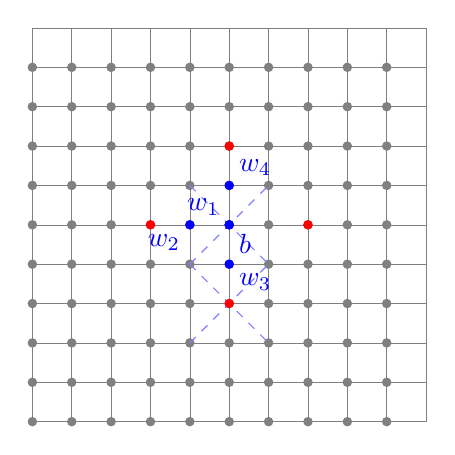
\begin{tikzpicture}[scale=0.5]
    % Draw the grid
    \draw[help lines] (0,0) grid (10,10);
    
    % Draw the vertices
    \foreach \x in {0,...,9} {
        \foreach \y in {0,...,9} {
            \filldraw[gray] (\x,\y) circle (3pt);
        }
    }
    
    % Draw the dashed lines
    \draw[dashed, blue!50] (4,4) -- (6,6);
    \draw[dashed, blue!50] (4,4) -- (6,2);
    \draw[dashed, blue!50] (4,6) -- (6,4);
    \draw[dashed, blue!50] (4,2) -- (6,4);
    
    % Draw the central vertex with labels
    \filldraw[blue] (5,5) circle (3pt) node[below right] {$b$};
    \filldraw[blue] (5,5) circle (3pt) node[above left] {$w_1$};
    \filldraw[blue] (4,5) circle (3pt) node[below left] {$w_2$};
    \filldraw[blue] (5,4) circle (3pt) node[below right] {$w_3$};
    \filldraw[blue] (5,6) circle (3pt) node[above right] {$w_4$};
    
    % Circle the qubits contributing to the phase difference
    \filldraw[red] (3,5) circle (3pt);
    \filldraw[red] (7,5) circle (3pt);
    \filldraw[red] (5,3) circle (3pt);
    \filldraw[red] (5,7) circle (3pt);
    
\end{tikzpicture}

\end{document}